Detached from the noise model, the goal of image denoising is to estimate the true image $X$ from the noisy observation $Y$. Let $\mathbf{i} = [i_1, i_2, \dots, i_d]^T$ be a column vector that defines the coordinates of each voxel in a \textit{d}-dimensional image space. In the most general form, $Y_{\mathbf{i}}$ is a mapping of $X_{\mathbf{i}}$ through a function $\mathcal{F}$:
\begin{equation*}
    Y_{\mathbf{i}} = \mathcal{F} (X_{\mathbf{i}})
\end{equation*}
where $Y_{\mathbf{i}}$ and $X_{\mathbf{i}}$ represent the noisy observation and the corresponding true image value at voxel $\mathbf{i}$, respectively. And the function $\mathcal{F}$ can vary depending on the noise model (e.g., additive or multiplicative noise, etc.).

The inverse problem is then to estimate $X$ from $Y$ (denoising), which is an ill-posed problem, meaning that there are multiple possible solutions for $X$ that could generate $Y$.

Denoising of images has been explored in both the spatial and transform domains. In the spatial domain, various linear and non-linear filtering techniques can be seen that utilize different kernels to manipulate pixel values directly. Linear filters, such as the mean filter, compute the average of pixel values within a neighborhood, smoothing the image but often blurring edges. Non-linear filters, like the median filter, replace each pixel with the median value of its neighbors, making them particularly effective for removing salt-and-pepper noise while preserving edges. Wiener filtering is another example, operating on statistical principles. The \gls{MSE} between the estimated and true image is minimized, adjusting the filter response according to the local image variance. This makes Wiener filtering particularly effective for Gaussian noise, as it can adaptively filter based on the estimated noise level and the signal characteristics, often resulting in superior denoising performance compared to simpler linear methods. More advanced non-linear methods, such as bilateral filtering, combine spatial proximity and intensity similarity, allowing for selective smoothing that retains sharpness around edges.

In addition to these filtering techniques, many denoising methods leverage prior knowledge about image characteristics, which significantly enhances their effectiveness. Common priors include assumptions about sparsity, smoothness, and texture. For example, total variation (TV) denoising assumes that natural images exhibit piece-wise smoothness, enabling the algorithm to preserve edges while reducing noise in flat regions. This method minimizes the total variation of the image, resulting in a denoised image that maintains important structural information. Similarly, non-local means (NLM) denoising capitalizes on the redundancy of similar patches within the image, estimating the value of a pixel based on a weighted average of other pixels with similar local structures, regardless of their spatial distance. By employing these priors, denoising algorithms can effectively exploit the inherent properties of images, leading to improved visual quality and more accurate representations of the true scene. Overall, the combination of spatial and transform domain techniques, along with the integration of prior knowledge, forms a robust framework for tackling the challenges of image denoising.


\section{Application to MPES data}
As described in section~\ref{section:datasets}, a 3D image is formed by binning over the three physical axes $k_x$, $k_y$, $E$ from different datasets such as \gls{GrIr} dataset. This data, while having the longest acquisition time still has a low average count of $\approx$1.05 counts per voxel. This makes the task of evaluation with reference metrics challenging as the true image is not available. Therefore, we look at different metrics to see which one is most reliable for the task.

To evaluate the performance of the denoising algorithms, the criteria needs to be defined. The ideal denoising would produce a distortion-free image, one free from artifacts and removing all unwanted signal. That is why simple linear filtering approaches do not work well, because they tend to blur the image, removing the features of interest, while removing noise.

\gls{IQA} is a field dedicated to measuring the objective and perpetual quality of an image. Objective metrics such as \gls{PSNR}, \gls{SSIM}, \gls{MSE} and \gls{MSSSIM} require a reference image---the true image---to compare the denoised image against. No reference metrics also exist, such as \gls{NIQE}, and subjective metrics such as the \gls{MOS}.

\begin{figure}[h]
    \centering
    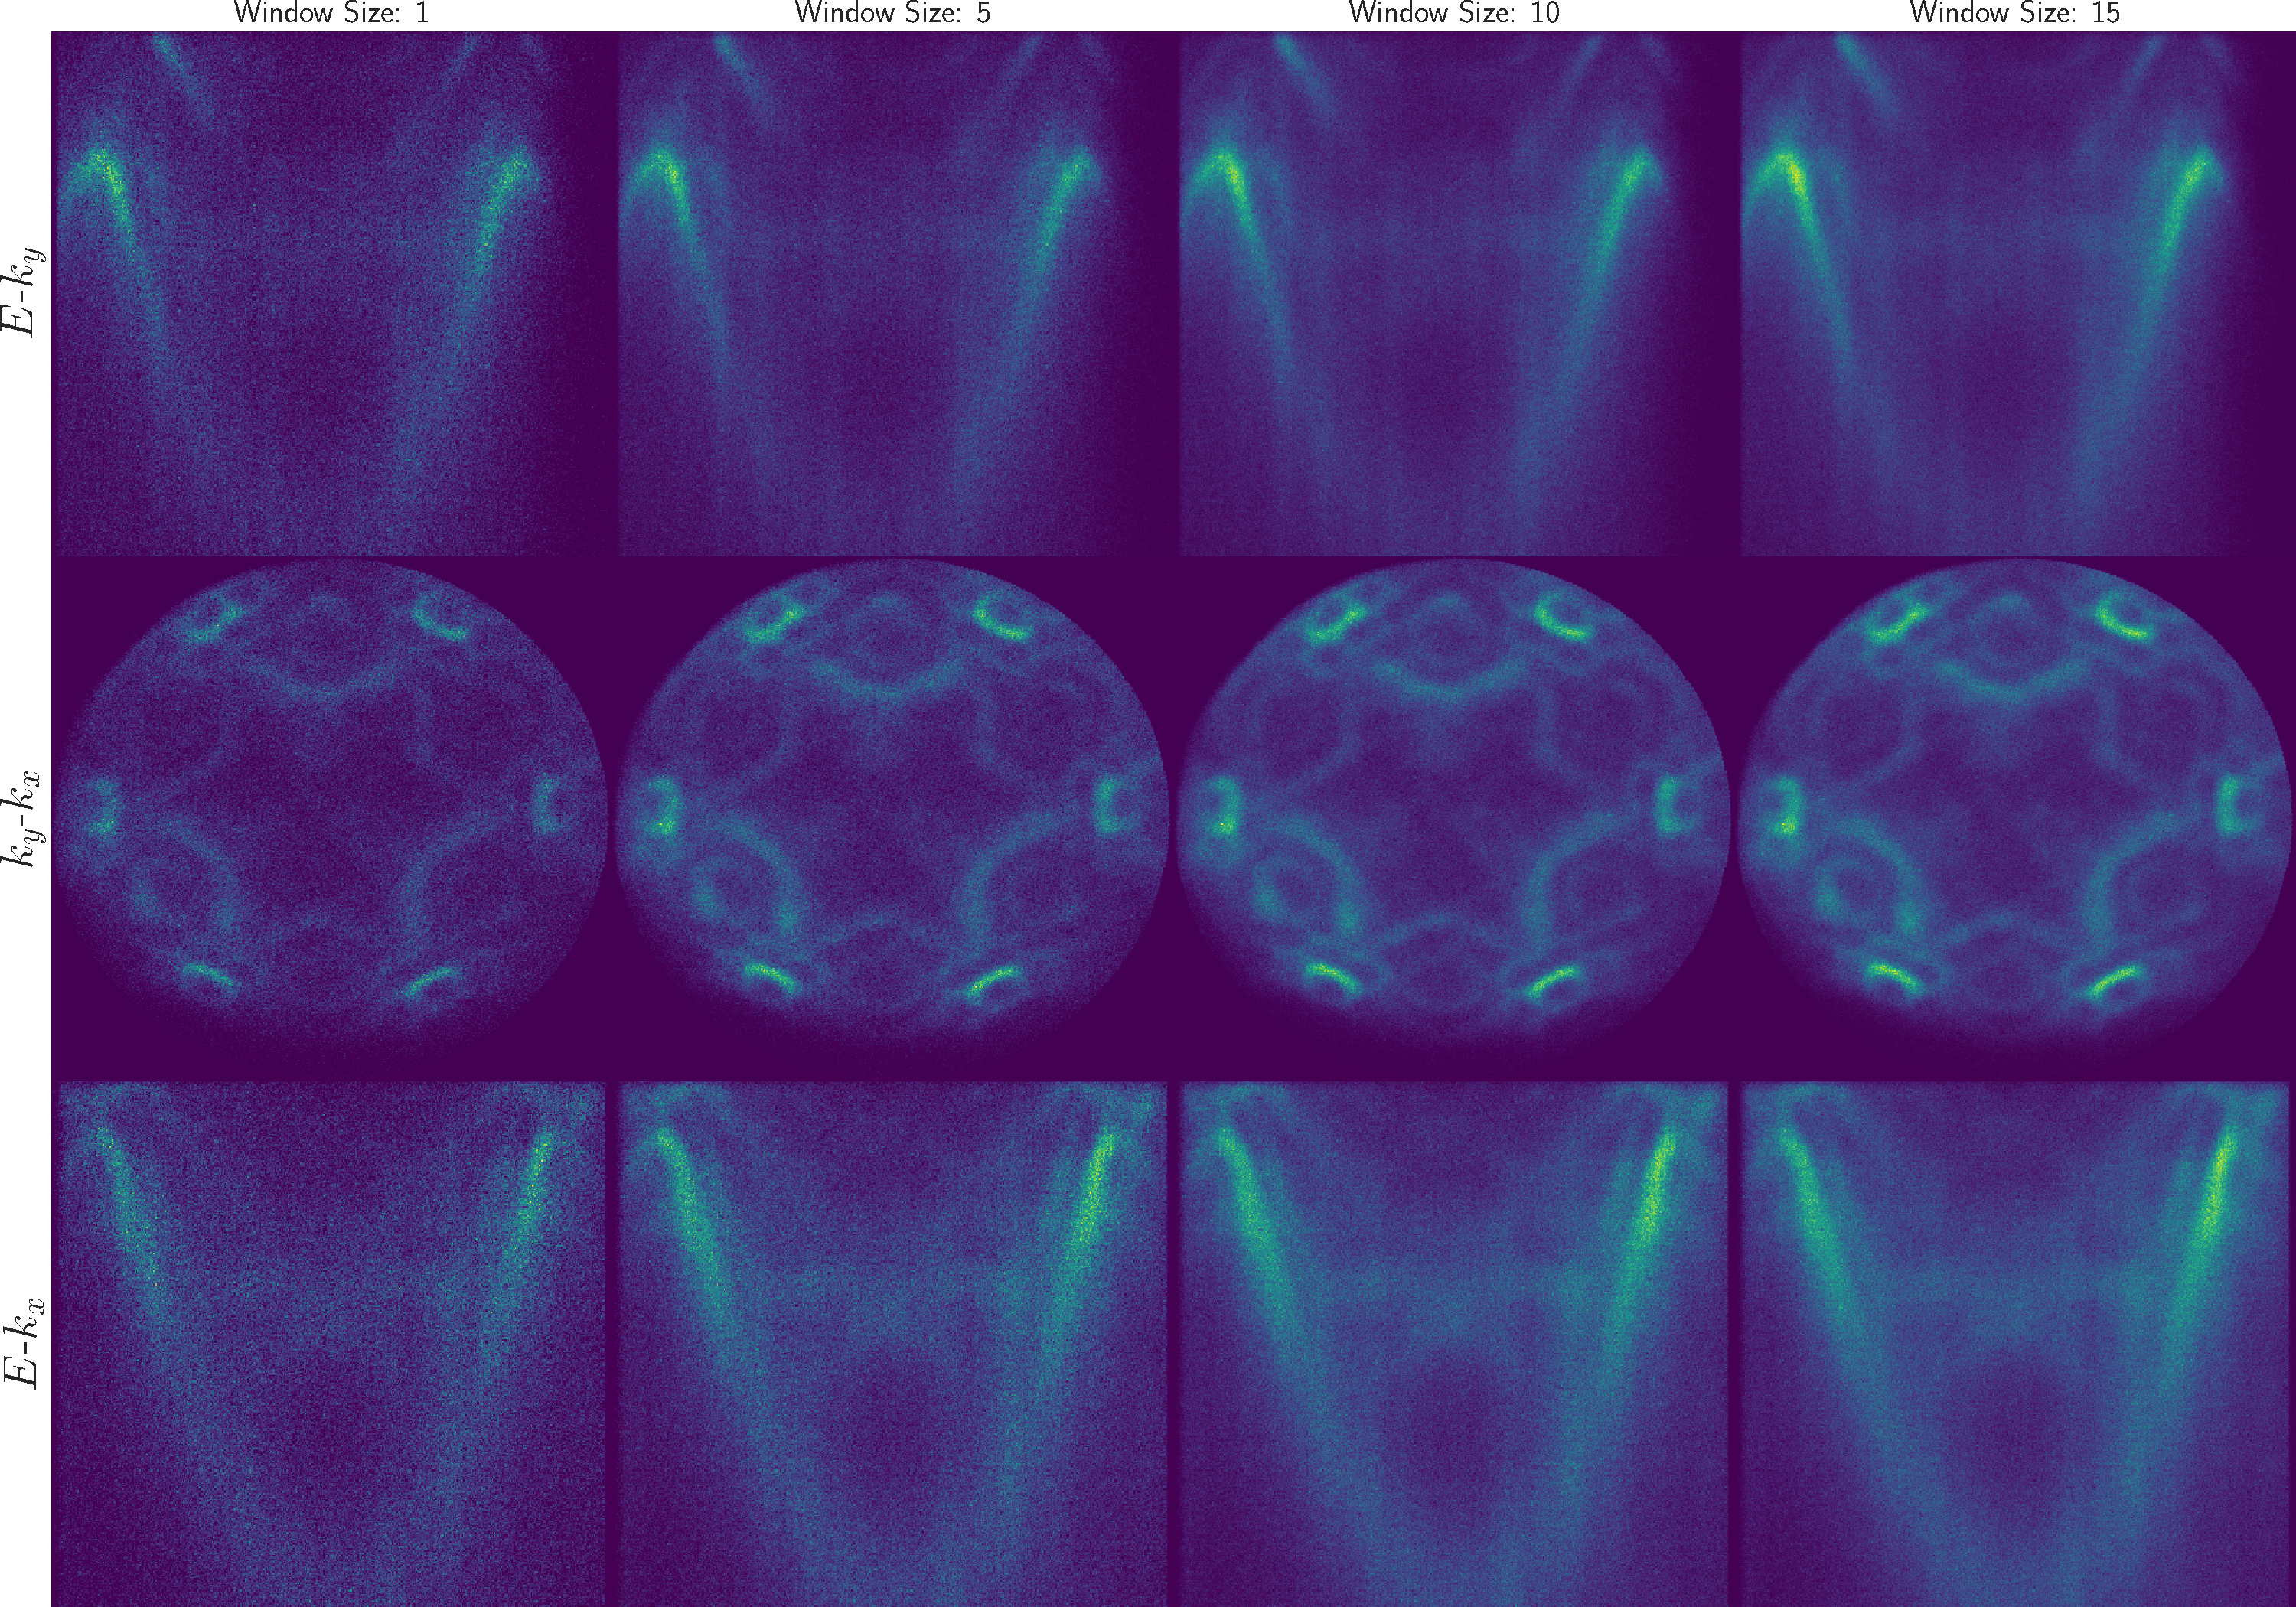
\includegraphics[width=1\linewidth]{images/slices.pdf}
    \caption{$E$-$k_x$ slices at arbitrary positions of the 3D \gls{GrIr} 3D dataset, showing the effect of averaging across different window sizes. The leftmost column shows a single slice with significant noise, while subsequent columns show slices averaged over windows of 5, 10, and 15 voxels. Increasing the window size progressively reduces noise, at the cost of broadening the features and reduced resolution.}
    \label{fig:slices}
\end{figure}

Given that even the high-count dataset exhibits a relatively low average count of approximately \num{1.05} counts per voxel, one method to create a high quality reference image is to average the neighboring slices. Figure~\ref{fig:slices} illustrates such a case, where it is evident that an ideal, noise-free reference image is not obtainable, even when averaging the neighboring slices. While the individual slice images are affected by noise, the window-averaged images, though exhibiting reduced spatial resolution, offer a marginal improve the noise.

Throughout the text, the images are always normalized to their maximum value in the [\numrange{0}{1}] range, as of interest are not the absolute intensity differences but rather the features and structures in the image.

In Appendix~\ref{sec:metric_comparison_experiment}, we compare the performance of different metrics (\gls{PSNR}, \gls{SSIM}, \gls{MSE} and \gls{MSSSIM}) for evaluating the denoising performance. It is found that the \gls{MSSSIM} metric is particularly well-suited for evaluating the denoising performance of images, when comparing against a noisy reference image. The \gls{MSSSIM} metric, conceived by \citeauthor{wangMultiscaleStructuralSimilarity2003} \cite{wangMultiscaleStructuralSimilarity2003}, extends SSIM by incorporating multiple scales. 

\section{BM3D: Denoising in Sparse Domain}

A lot of the earlier algorithm assume the noise prior to be additive noise. This can be written as:
\begin{equation}
    Y = X + N
\end{equation}
and many more assume the noise to be \gls{AWGN} with noise of form in equation~\ref{eq:awgn}. This is because the normal distribution has nice mathematical properties, allowing to derive theoretical guarantees.

\begin{equation}\label{eq:awgn}
    N \sim \mathcal{N}(0, \sigma^2)
\end{equation}

One such \gls{AWGN} denoising algorithm is the celebrated \gls{BM3D} algorithm, introduced first by \citeauthor{dabovImageDenoisingSparse2007} in \cite{dabovImageDenoisingSparse2007}, building upon many of the classical denoising techniques such as the transform domain denoising, non-local means and filtering methods (such as the Wiener filter). As shown in see Algorithm~\ref{alg:bm3d}, the proposed scheme works by grouping similar patches in a 2D image and applying a 3D transform\footnote{This algorithm has also been proposed for 3D images, dubbed BM4D.}. This leads to an enhanced sparse representation of the image which after filtering is transformed back to the spatial domain.
% Main BM3D Algorithm
\begin{algorithm}
    \caption{BM3D Denoising Algorithm}\label{alg:bm3d}
    \begin{algorithmic}[1]
    \Require Noisy image $I$
    \Ensure Denoised image $I_{\text{denoised}}$
    \Statex
    \Procedure{BM3D}{$I$, $\sigma^2$}
        \State $I_{\text{denoised}} \gets I$
        
        \For{each reference block $B_r$ in $I$}
            \State $\mathcal{B} \gets \textsc{Grouping}(B_r)$
            \State $B_{\text{filtered}} \gets \textsc{CollaborativeFiltering}(\mathcal{B})$
            \State Aggregate $B_{\text{filtered}}$ into $I_{\text{denoised}}$
        \EndFor
        
        \State \textbf{return} $I_{\text{denoised}}$
    \EndProcedure
    \end{algorithmic}
\end{algorithm}

In the Grouping step, blocks who are the least dissimilar to the reference block $B_r$ are used. The dissimilarity measure used is the $l^2$-distance. The Collaborative Filtering\footnote{Interestingly, collaborative filtering has been the backbone of recommendation systems such as by Netflix and Spotify.} shown in Algorithm~\ref{alg:collaborativefiltering} is then applied to the grouped blocks. This step consists of a 3D transform such as the discrete cosine transform (or the wavelet transform can be used). A filter is applied to the transformed blocks to remove noise, initially by hard thresholding and in the second run by Wiener filtering. The inverse 3D transform is then applied to the filtered blocks, and the filtered blocks are aggregated to form the estimate. The first run is considered the basic estimate, and it is only after Collaborative Wiener filtering that the final estimate is obtained.
    
% Collaborative Filtering Algorithm
\begin{algorithm}
    \caption{Collaborative Filtering}\label{alg:collaborativefiltering}
    \begin{algorithmic}[1]
    \Require Group of similar blocks $\mathcal{B}$
    \Ensure Filtered block $B_{\text{filtered}}$
    \Procedure{CollaborativeFiltering}{$\mathcal{B}$}
        \State Apply 3D transform (e.g., DCT) to $\mathcal{B}$
        \State Apply filtering (hard thresholding or Wiener)
        \State Perform inverse 3D transform
        \State Aggregate filtered blocks
        \State \textbf{return} $B_{\text{filtered}}$
    \EndProcedure
    \end{algorithmic}
\end{algorithm}

The \gls{BM3D} algorithm had showed one of the best denoising performances and can only be contested by the recent deep-learning based denoising methods. 

\section{Poisson Noise Model}\label{sec:poisson-noise-model}
In the case of photoelectron counting, the observed intensity $Z_{\mathbf{i}} \in \mathbb{Z}_{\geq 0}$ at each voxel (with $\mathbf{i} = [i_1, i_2, \dots, i_d]^T$ the coordinate vector in $d$-dimensional space) can be modeled as a Poisson random variable with parameter $Y_{\mathbf{i}}$. This is shown in Section~\ref{section:photoelectron-counting-stats} to be true for a constant intensity light source. The relation can be expressed as: $Z_{\mathbf{i}} \sim \text{Poi}(Y_{\mathbf{i}})$

\begin{equation}
    P(Z_{\mathbf{i}} = z| Y_{\mathbf{i}} = y) = \frac{y^z e^{-y}}{z!}
\end{equation}


Here, $z$ represents the observation at voxel $i$, while $y$ corresponds to the expected number of detected electrons, the underlying intensity that we aim to recover. Formally $\mathbb{E}[Z_{\mathbf{i}} | Y_{\mathbf{i}}] = Y_{\mathbf{i}}$

The Poisson noise can then be written as:
\begin{equation}
    N_{\mathbf{i}} = Z_{\mathbf{i}} - \mathbb{E}[Z_{\mathbf{i}} | Y_{\mathbf{i}}]
\end{equation}

This noise is signal dependent as the variance is dependent on the true signal $Var[N_{\mathbf{i}} | Y_{\mathbf{i}}] = [Z_{\mathbf{i}} | Y_{\mathbf{i}}] = Y_{\mathbf{i}}$ and hence it can be seen that the with decreasing intensity, the noise increases.

\section{Variance Stabilization Transform: Anscombe}
\Glspl{VST} is used to map the values of the data to a new domain so that the variance becomes constant. In \cite{anscombeTransformationPoissonBinomial1948} introduced such a \gls{VST} for data distributed according to the Poisson, Binomial, and Negative Binomial distributions. The Anscombe transform is defined as:
\begin{equation}
    f(Z) = 2 \sqrt{Z + \frac{3}{8}}
\end{equation}

Applying this to a Poisson distributed random variable gives a signal whose noise is asymptotically additive standard normal. This transformed data can then be denoised using \gls{AWGN} denoising techniques such as \gls{BM3D}. Denoising $f(Z)$ produces a signal $\mathcal{D}$ that is an estimate for $\mathbb{E}[f(Z) | Y]$, with $Y$ being the true signal. Hence, the final estimate for the true signal $Y$ can be obtained by applying the inverse Anscombe transform to $\mathcal{D}$.

\begin{algorithm}
    \caption{Algorithm to Denoise Poisson Corrupted Images}\label{alg:anscombe-bm3d}
    \begin{algorithmic}[1]
    \Require Noisy image $I$
    \Ensure Denoised image $I_{\text{denoised}}$
    \Statex
    \Procedure{AnscombeBM3D}{$I$, $\sigma^2$}
        \State $I_{\text{anscombe}} \gets \textsc{AnscombeTransform}(I)$
        
        \State $I_{\text{bm3d}} \gets \textsc{BM3D}(I_{\text{anscombe}}, \sigma^2, b, W, \tau)$
        
        \State $I_{\text{denoised}} \gets \textsc{InverseAnscombeTransform}(I_{\text{bm3d}})$
        
        \State \textbf{return} $I_{\text{denoised}}$
    \EndProcedure
    \end{algorithmic}
\end{algorithm}

Since the transformation is non-linear, an algebraic inverse is biased. \citeauthor{makitaloOptimalInversionAnscombe2011} \cite{makitaloOptimalInversionAnscombe2011} proposed an exact unbiased inverse of $\mathbb{E}[f(Z) | Y]$ giving the denoised estimate $\mathbb{E}[Z | Y]$. This method performs better than methods based on explicit Poisson noise removal. Therefore, in the next few sections we make use of the scheme described in Algorithm~\ref{alg:anscombe-bm3d} to denoise 2D slices from the \gls{MPES} data.

\section{Finding the Optimal Sigma}
Let us start with attempting to denoise the noisy realization with \num{1.6e7} electron counts of the $k_y$-$k_x$ images shown in Figure~\ref{fig:slices}, as the target has clear features to compare against. We use the Anscombe--\gls{BM3D}--Inverse Anscombe scheme described above. Single slice and window-averaged images \numlist{1;5;10;15} are compared against the reference (single slice and window-averaged of the \num{1.86e8} counts dataset) using the \gls{MSSSIM} metric. The value of $\sigma$ is arbitrarily set to \num{0.2}. One example of noisy, denoised, and target images is shown in Figure~\ref{fig:noisy-denoised-ref-16M-avg-bm3d}, with the noisy image formed by averaging 5 $k_y$-$k_x$ slices and the target image formed by averaging 15 $k_y$-$k_x$ slices.

\begin{figure}[h]
    \centering
    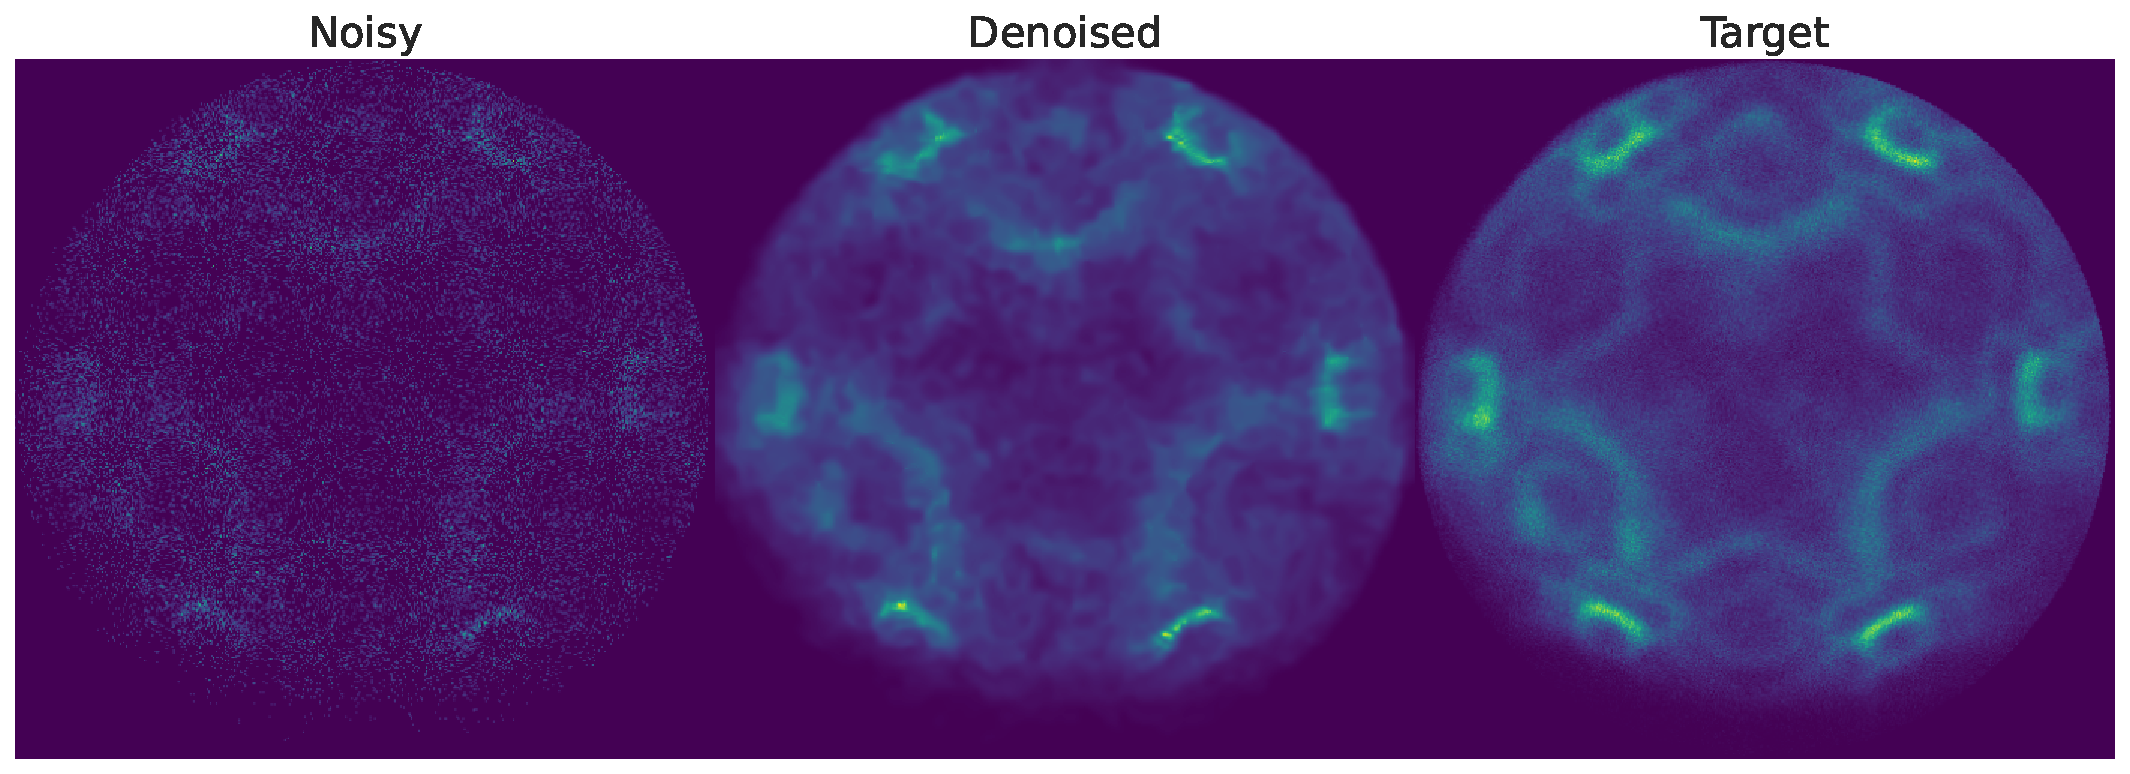
\includegraphics[width=1\linewidth]{images/noisy_denoised_ref_16M_avg_bm3d.pdf}
    \caption{Noisy and target images formed from averaging 5 and 15 $k_y$-$k_x$ slices, respectively. The figure shows the noisy, denoised, and target images, with the denoising performed using the \gls{BM3D} with Anscombe. \gls{MSSSIM} reports \num{0.85} when compared against this target.}
    \label{fig:noisy-denoised-ref-16M-avg-bm3d}
\end{figure}


Using a confusion matrix, Figure~\ref{fig:confusion_matrix_msssim_window_avg} shows how the metric changes when varying window sizes. It becomes evident that a larger window size yields a better comparison for denoising. This is because the larger window size reduces the noise in the target image, making the comparison more accurate. Denoising single slice images leads to generally poor results, highlighting that for low count images, this scheme is insufficient.

\begin{figure}[h]
    \centering
    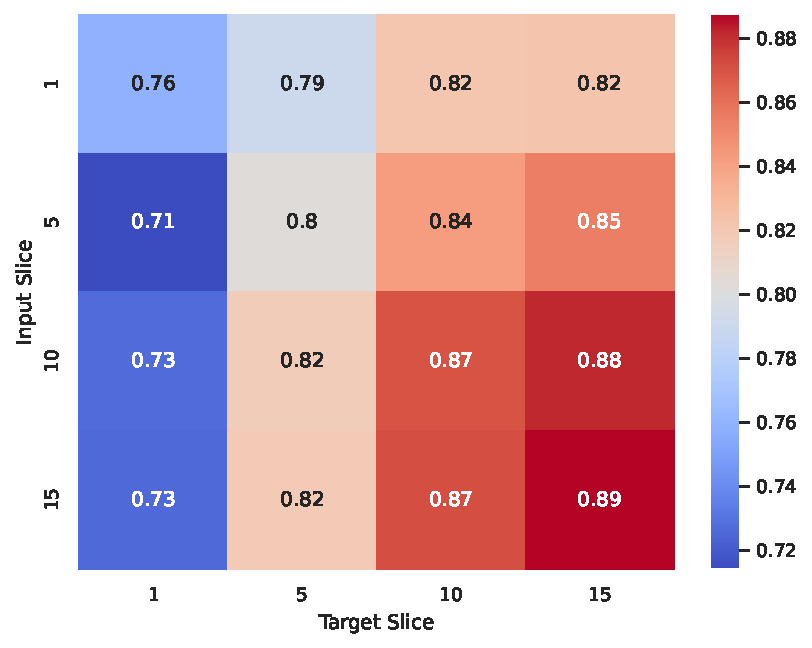
\includegraphics[width=0.5\linewidth]{images/confusion_matrix_msssim_window_avg.pdf}
    \caption{Confusion matrix showing the \gls{MSSSIM} values for different window-averaged input and target images. The \gls{MSSSIM} is computed for the denoised images using the Anscombe--\gls{BM3D}--Inverse Anscombe scheme. The matrix shows that using a larger window for target image leads to better comparison of denoising.}
    \label{fig:confusion_matrix_msssim_window_avg}
\end{figure}

Till now, we only looked at a single count rate and denoising with a single $\sigma$ value. However, considering that the noise decreases with increased electron counts, the expectation would be that the level of denoising required also decreases. One way would be to estimate the noise level and use that estimate as the $\sigma$ for denoising. A different approach would be to perform a constrained optimization to find optimal $\sigma$ denoted $\sigma_{\text{oo}}$, such that the metric \gls{MSSSIM} is maximized. For user defined parameters to an algorithm, this sort of optimization is known as a hyperparameter search. An exhaustive grid search is the simplest method, but it is computationally expensive. Therefore, we use \texttt{optuna}, which performs Bayesian optimization to find the optimal parameters, optimizing for \num{50} trials. The search is performed on \num{10} window-averaged 2D image slices (same as in Figure~\ref{fig:noisy-denoised-ref-16M-avg-bm3d}) with 5 different noisy realizations for each count.


\begin{figure}[h]
    \centering
    % First subfigure (Hyperparameter Search with Averaged 10 Images using MS-SSIM)
    \begin{subfigure}[t]{0.49\linewidth}
        \centering
        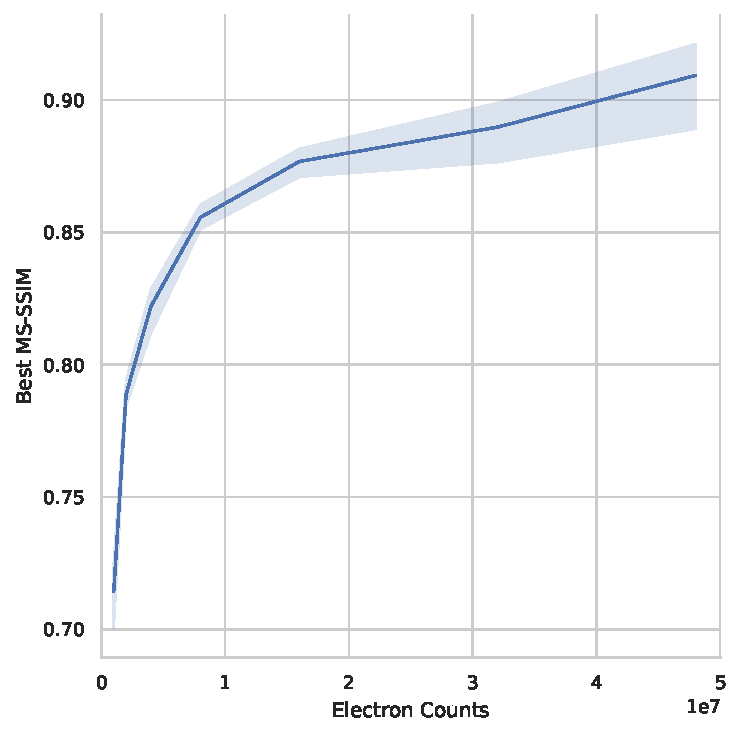
\includegraphics[width=\linewidth]{images/hyperparameter_msssim_averaged_10_images.pdf}
        \caption{Hyperparameter search results using MS-SSIM metric, averaged over 10 images.}
        \label{fig:hyperparameter-msssim-averaged-10-images}
    \end{subfigure}
    \hfill
    % Second subfigure (Hyperparameter Search with Averaged 10 Images using Sigma)
    \begin{subfigure}[t]{0.49\linewidth}
        \centering
        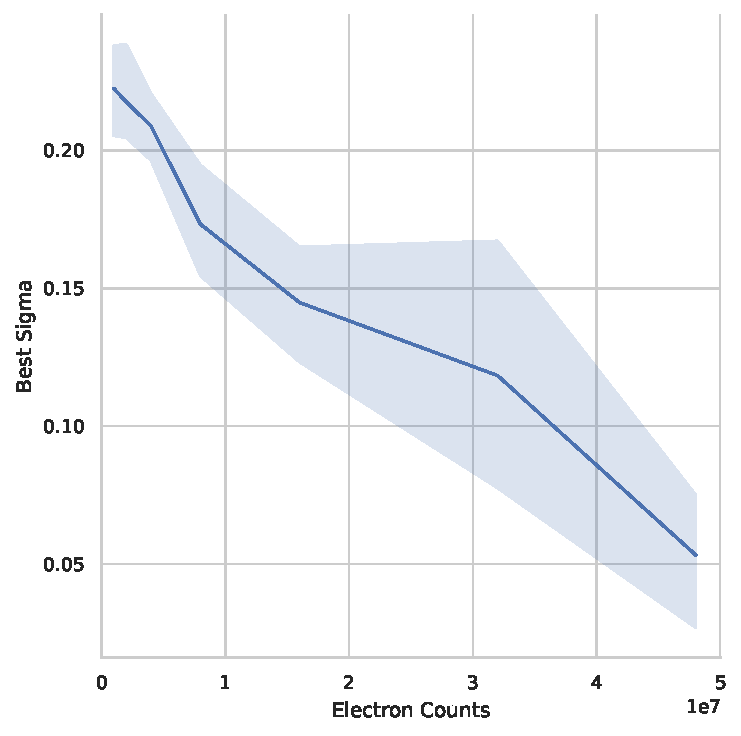
\includegraphics[width=\linewidth]{images/hyperparameter_sigma_averaged_10_images.pdf}
        \caption{Hyperparameter search results using Sigma metric, averaged over 10 images.}
        \label{fig:hyperparameter-sigma-averaged-10-images}
    \end{subfigure}
    \caption{Results of hyperparameter search for \gls{BM3D} $\sigma$ for different electron counts, using the \gls{MSSSIM} metric. The images are a window-average of \num{10} slices from the 3D volume.}
    \label{fig:hyperparameter-averaged-10-images}
\end{figure}

The results in Figure~\ref{fig:hyperparameter-averaged-10-images} corroborate the hypothesis that the optimal $\sigma$ for denoising decreases with increasing electron counts, a linearly decreasing trend.

While using \gls{MSSSIM} as the objective function for optimization is good at showing the denoising performance improvement, it leads to more cautious results (low $\sigma_{\text{oo}}$ values) as those fare better against the target, which has the relevant features but is also noisy. To counter that, we scale the optimum $\sigma_{\text{oo}}$ values by a factor of 2 to get a more aggressive denoising and denote that as $\sigma_{\text{o}}$ and use this for denoising. A comparison of the denoised image using the optimal $\sigma_{\text{o}}$ and the adjusted optimal $\sigma_{\text{oo}}$ is shown in Figure~\ref{fig:denoised-optimal-sigma}.

\begin{figure}[h]
    \centering
    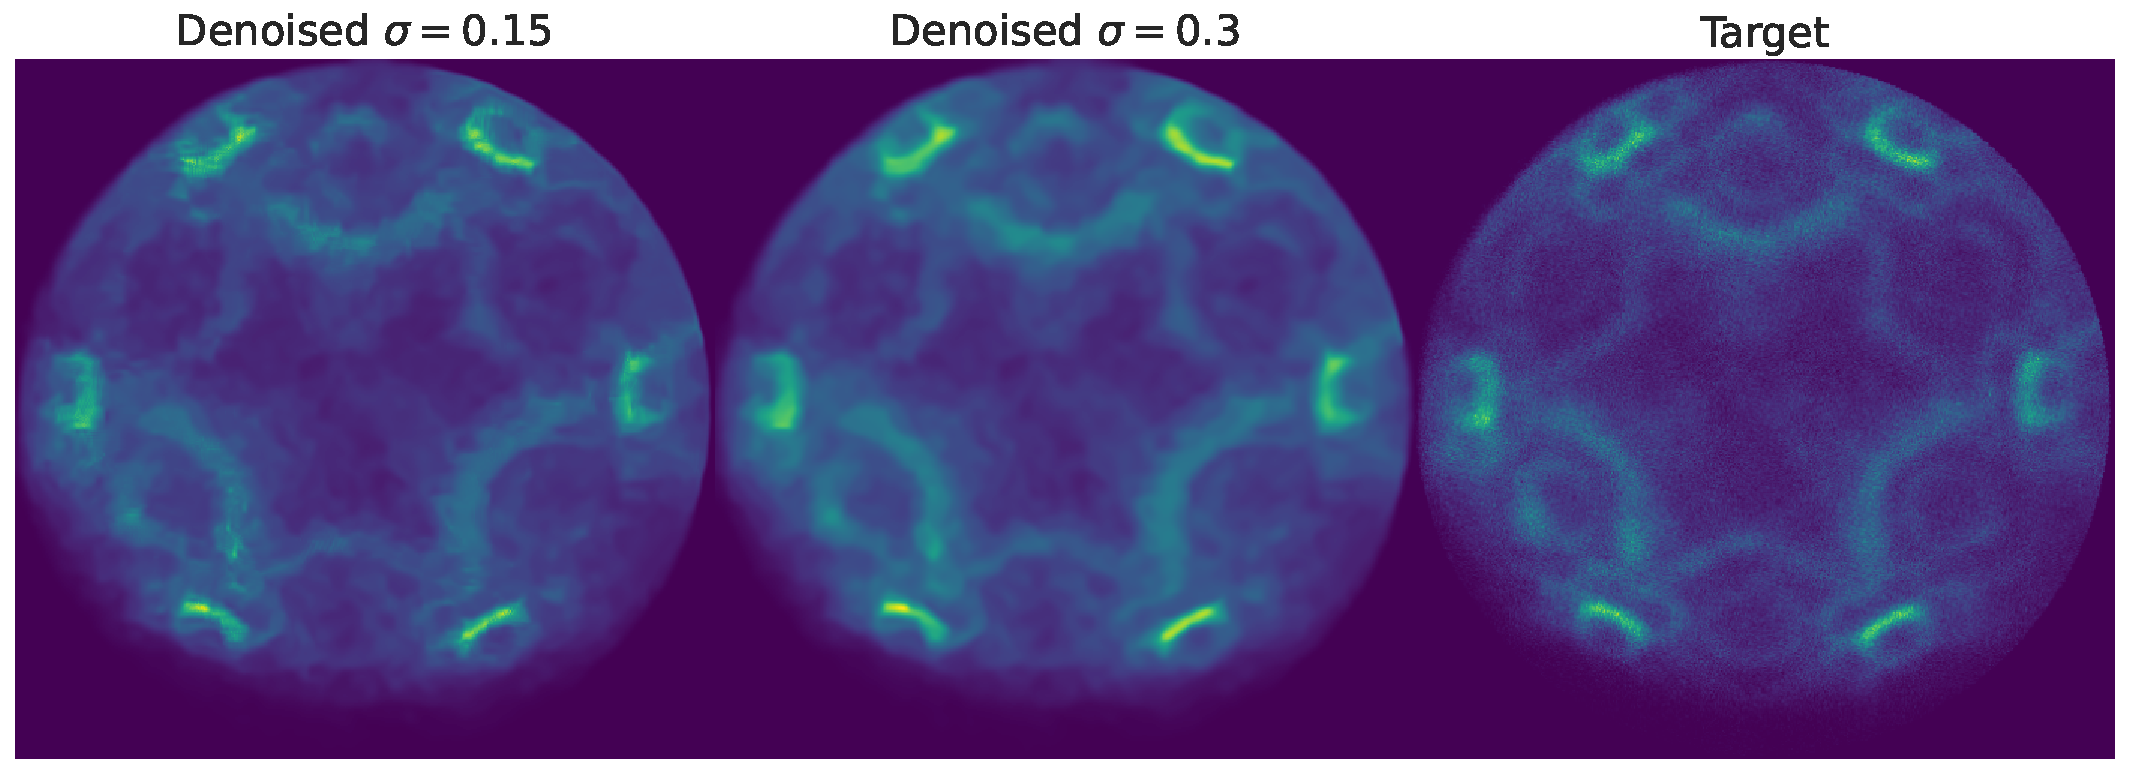
\includegraphics[width=1\linewidth]{images/denoised_optimal_sigma.pdf}
    \caption{Denoised image using the optimal $\sigma_{\text{oo}}=0.15$ (optimal value found for \num{1.6e7} counts from the hyperparameter search) denoised image with $\sigma_{\text{o}}=0.3$ (adjusted optimal value) and the target image.}
    \label{fig:denoised-optimal-sigma}
\end{figure}

The denoising performance below \num{4e6} is poor, with or without the optimal value $\sigma_{\text{oo}}$, and even though the \gls{MSSSIM} reports high values. Figures~\ref{fig:noisy-denoised-ref-2M-avg-bm3d} and \ref{fig:noisy-denoised-ref-4M-avg-bm3d} show the denoised images for \num{2e6} and \num{4e6} counts, with an average count of \num{0.14} and \num{0.27} in the noisy image, respectively, whereas the average count in target image is \num{12.9}. It can be seen that the perpetual quality of the denoised images is poor, with the features not being well-preserved. This highlights that \gls{BM3D} is not well suited for denoising such low count images.

\begin{figure}[h]
    \centering
    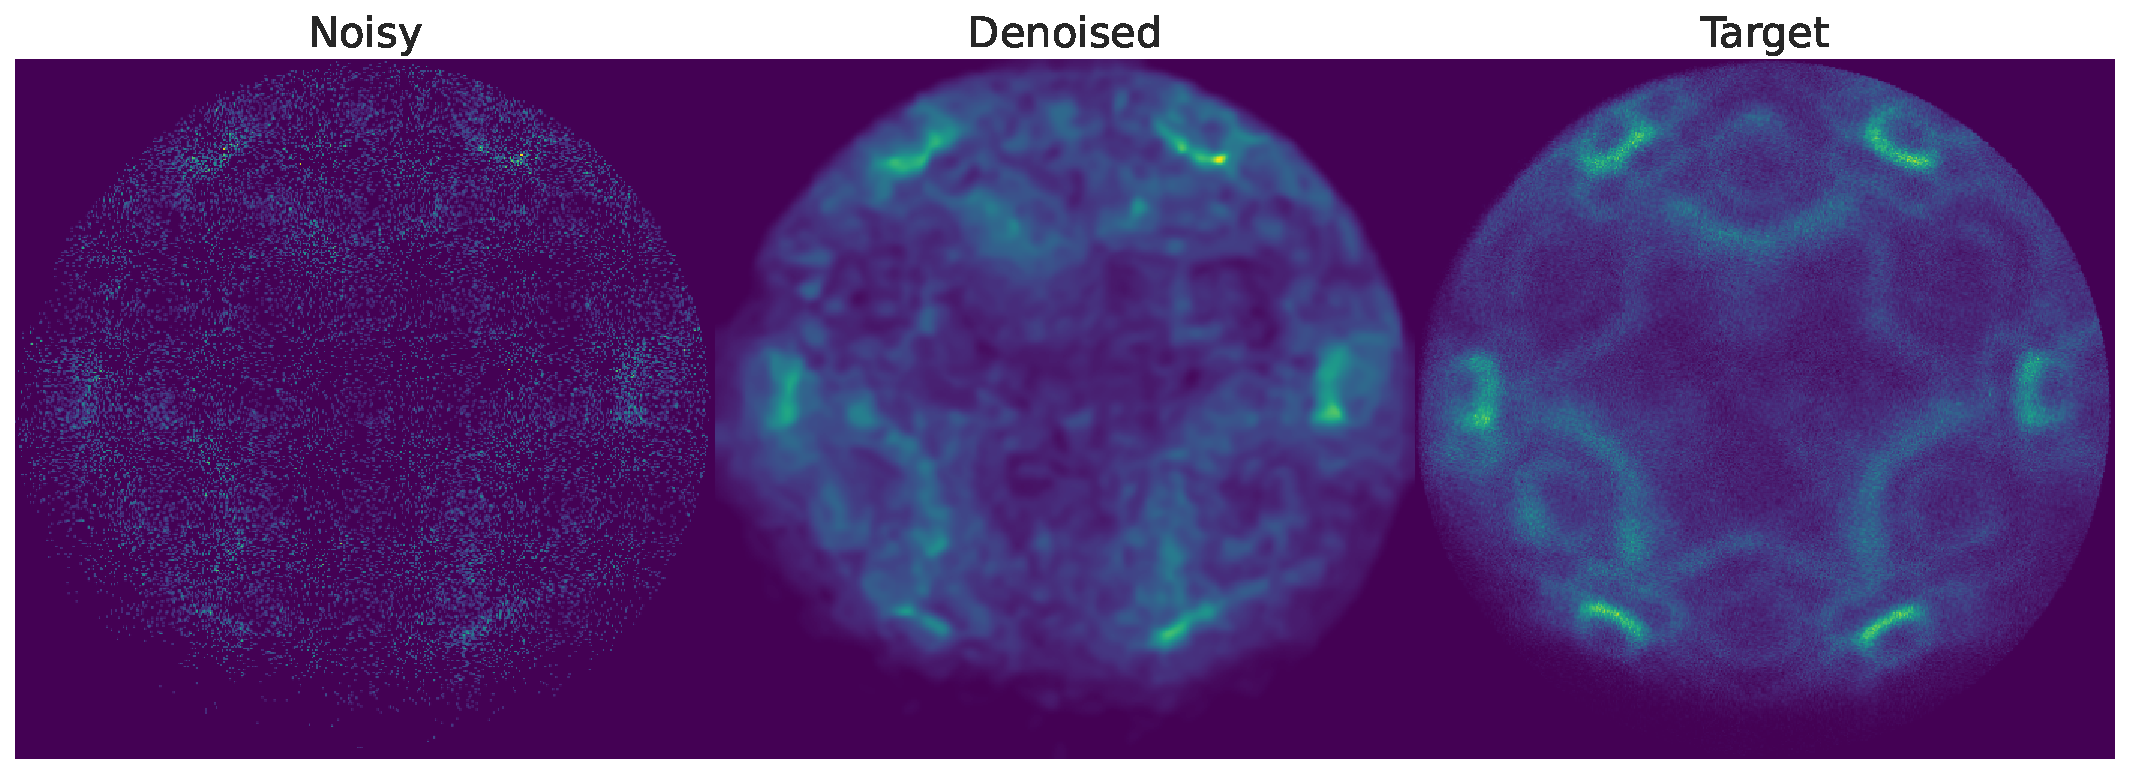
\includegraphics[width=1\linewidth]{images/noisy_denoised_ref_2M_avg_bm3d.pdf}
    \caption{Noisy and target images formed from averaging 10 $k_y$-$k_x$ slices of the \num{2e6} count dataset. The figure shows the noisy, denoised, and target images, with the denoising performed using the \gls{BM3D} with Anscombe. The denoising performance is quite poor, even with the adjusted optimal $\sigma_{\text{o}}\approx0.4$.}
    \label{fig:noisy-denoised-ref-2M-avg-bm3d}
\end{figure}


\begin{figure}[h]
    \centering
    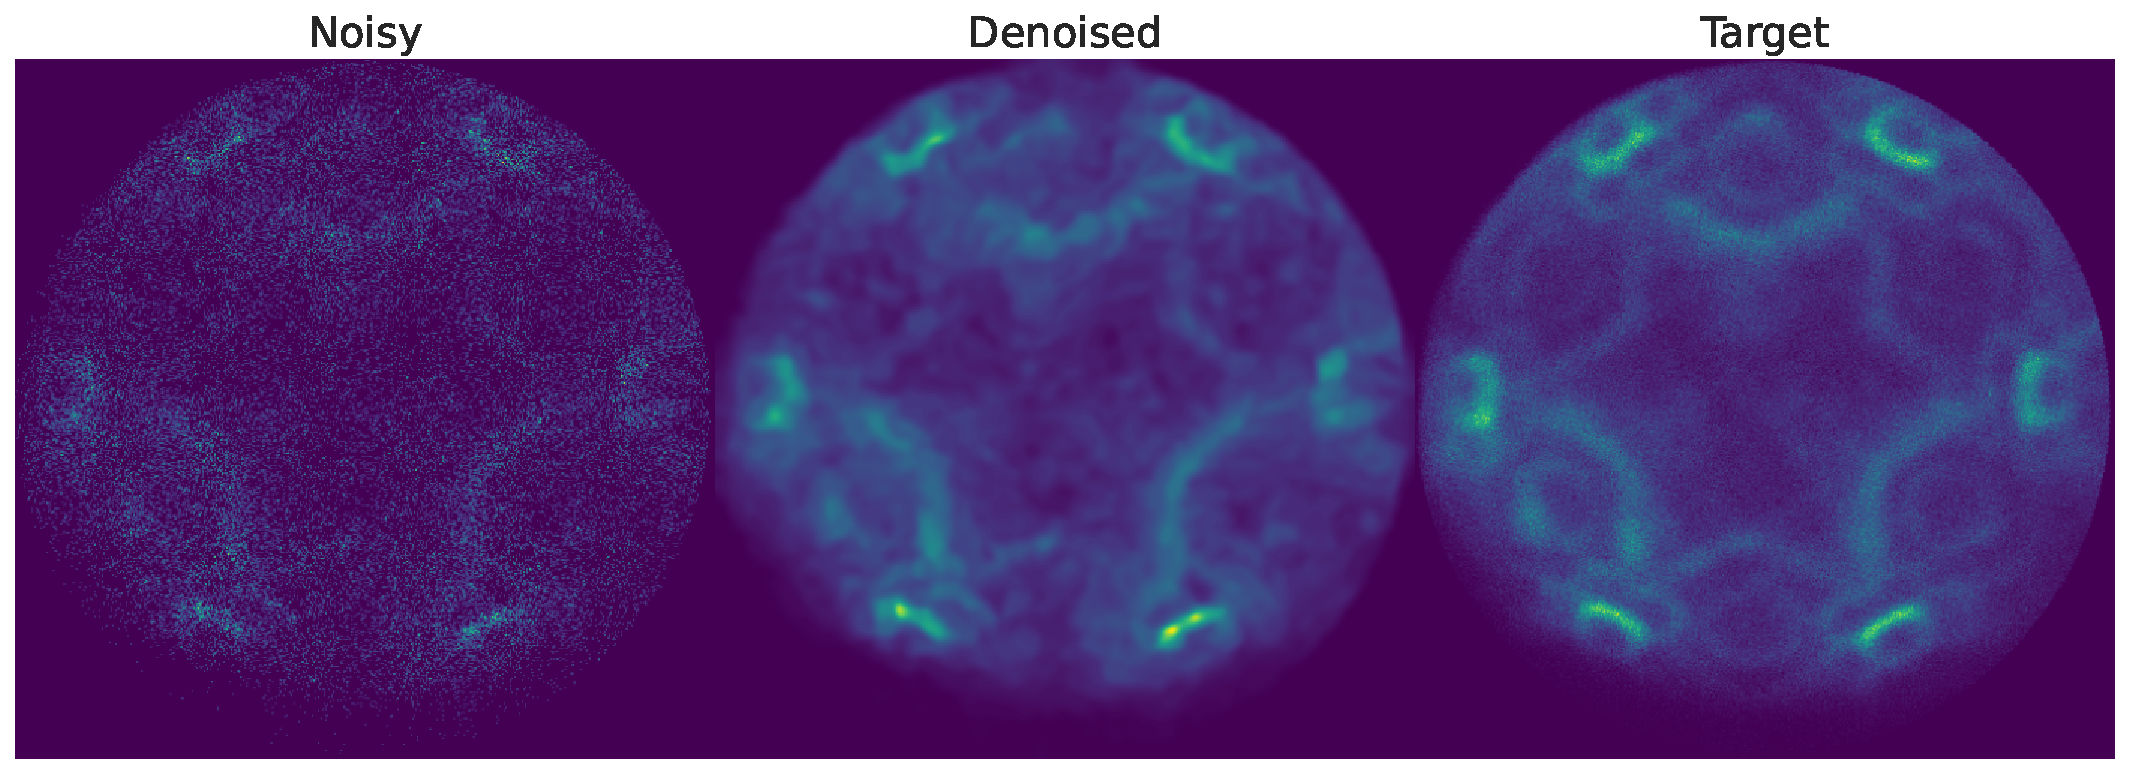
\includegraphics[width=1\linewidth]{images/noisy_denoised_ref_4M_avg_bm3d.pdf}
    \caption{Noisy and target images formed from averaging 10 $k_y$-$k_x$ slices of the \num{4e6} count dataset. The figure shows the noisy, denoised, and target images, with the denoising performed using the \gls{BM3D} with Anscombe. The denoising performance leaves room for improvement, even with the adjusted optimal $\sigma_{\text{o}}\approx0.4$.}
    \label{fig:noisy-denoised-ref-4M-avg-bm3d}
\end{figure}


We now evaluate the denoising performance of the \gls{BM3D} algorithm with the optimal $\sigma_{\text{o}}$ values found using the hyperparameter search. A total of \num{1847} images are extracted from datasets with counts \numlist{1e6;2e6;4e6;8e6;1.6e7;3.2e7;4.8e7}. The images are window-averages of 10 slices for both the noisy and target images. The baseline \gls{MSSSIM} is computed using the noisy image. The data in Figure~\ref{fig:bm3d-msssim} shows that objectively, there is an improvement in image quality with denoising up till \num{4e7} counts, with the \gls{MSSSIM} values increasing from \num{0.6} to \num{0.83}. When visually inspecting above that count, the denoised images show results better than the target, with the noisy target likely being the reason why the \gls{MSSSIM} values are lower. 

\begin{figure}[h]
    \centering
    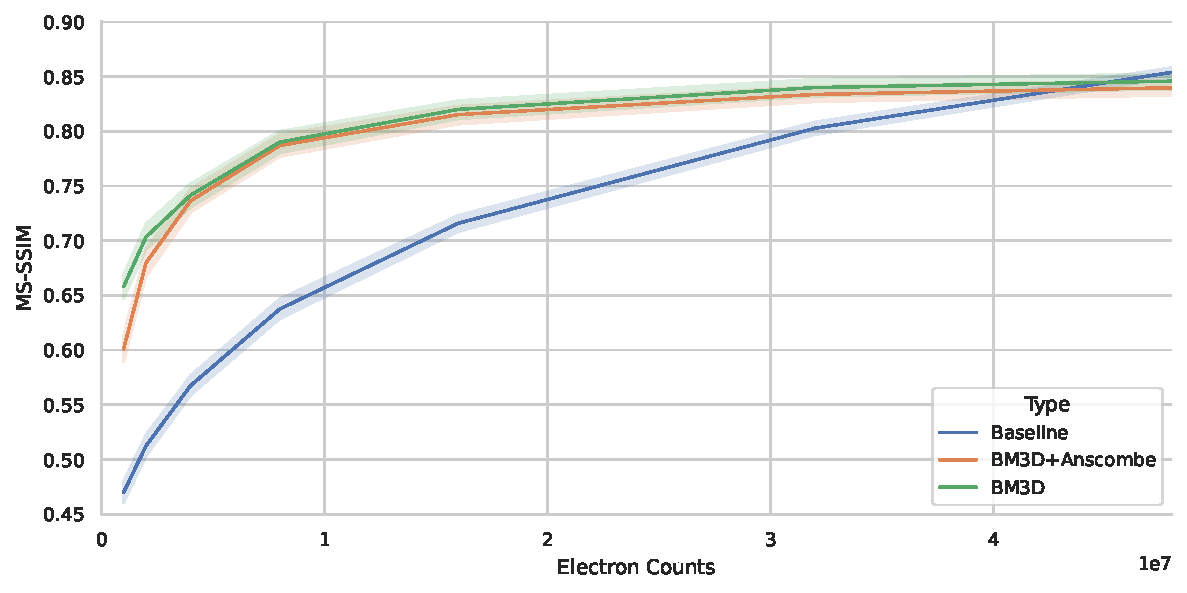
\includegraphics[width=0.7\linewidth]{images/bm3d_msssim.pdf}
    \caption{Denoising performance of the \gls{BM3D} algorithm with the optimal $\sigma_{\text{o}}$ values determined through the hyperparameter search. The images are window-averages of 10 slices for both the noisy and target images. The baseline metric is computed using the noisy image.}
    \label{fig:bm3d-msssim}
\end{figure}

We now evaluate the denoising performance of the \gls{BM3D} algorithm using the optimal $\sigma_{\text{o}}$ values determined through hyperparameter search. A total of \num{1847} images were extracted from two datasets, each with counts of \numlist{1e6;2e6;4e6;8e6;1.6e7;3.2e7;4.8e7}. These images are window-averaged over 10 slices for both the noisy and target images. The baseline \gls{MSSSIM} metric was computed using the noisy images. As shown in Figure~\ref{fig:bm3d-msssim}, there is a noticeable improvement in image quality with denoising up to \num{4e7} counts, with \gls{MSSSIM} values increasing from \num{0.6} to \num{0.83}. Beyond this count, visual inspection reveals that the denoised images appear better than the noisy target, which likely explains the lower \gls{MSSSIM} values.